\begin{figure*}[h]
    \centering
    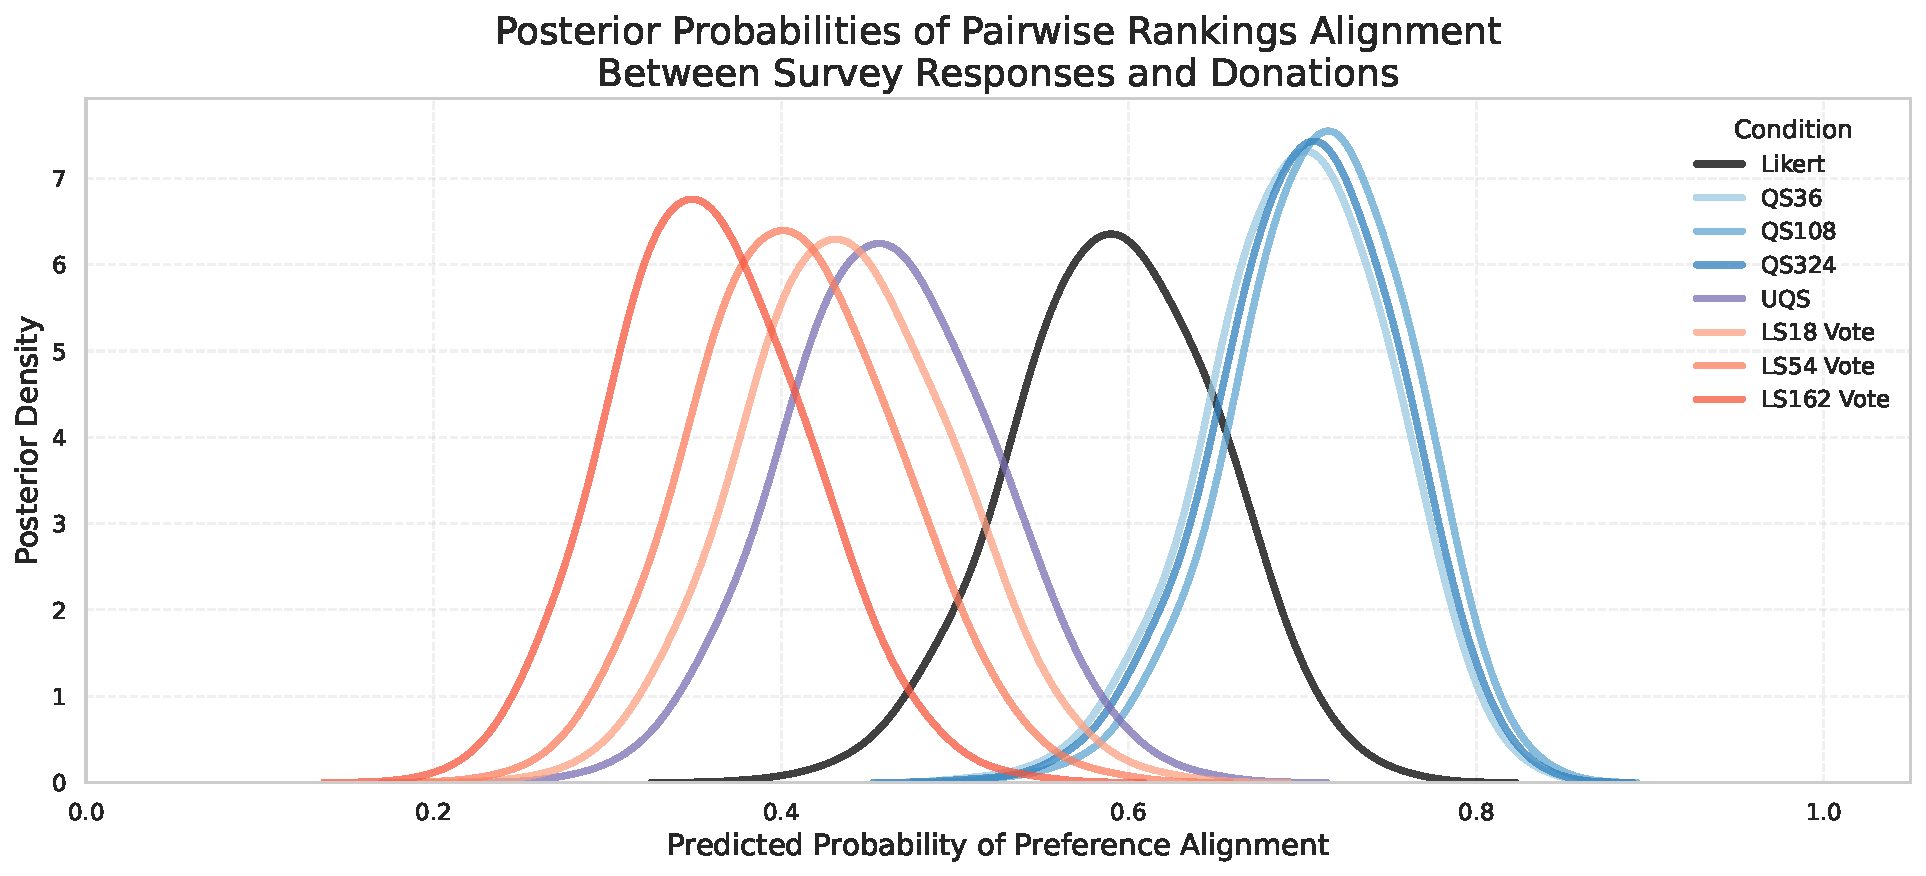
\includegraphics[width=\textwidth]{content/image/overlapping_density_custom_palette.pdf}
    \caption[]{
    This figure presents the posterior density distributions of the probability that pairwise rankings from various survey tools align with participants' actual donation behavior. The x-axis shows the predicted probability of correct pairwise ranking alignment, where 1 indicates perfect alignment. The y-axis represents the posterior density across the sampled distribution. Each curve corresponds to a different survey condition. QS with varying budgets cluster together, exhibiting higher alignment probabilities as reflected by their distributions peaking further to the right. In contrast, UQS and LS show lower alignment, with LS performance declining as its budget increases. \textbf{Main takeaway:} Budget-constrained QS elicit pairwise rankings that align more closely with participants' donation behaviors, highlighting their effectiveness in capturing directional preferences.}
    \label{fig:ranking_posterior}
\end{figure*}

\subsection{Pairwise Preference Ranking Results}
\label{sec:result_1}

\textbf{Results interpretation: }To evaluate how well a survey tool reflects a participant's preference ranking between two causes, we calculate the posterior distribution of the probability that the pairwise preference ranking reflected through a survey tool aligns with that reflected in donation amounts (\Cref{fig:ranking_posterior}). Furthermore, we compare survey tools' abilities to elicit accurate pairwise preference rankings using the odds ratio of the predicted odds of alignment between survey and donation preference rankings. For instance, an odds ratio of 2 between survey tools A and B means that the odds of participants expressing the same preference rankings in survey tool A and donations is twice those of participants using survey tool B. We say that two survey tools differed significantly when the 94\% Highest Posterior Density Interval (HPDI) of the odds ratio's posterior distribution does not include the reference value of 1 (odds ratio = 1 means having the same odds). 

\textbf{QS outperformed the Likert scale survey in eliciting preference rankings consistent with donations, with a small effect size} (odds ratio mean = 1.65, 94\% HPDI = [1.55, 1.76])\footnote{Odds ratio = 1.68, 3.47, 6.71 corresponds to a small, medium, and large effect size, respectively~\cite{chen2010big}}. The model predicted that a participant's preference ranking in QS aligned with that in donations with a 70\% chance on average, higher than the 59\% average probability for the Likert scale survey. 

\textbf{When the budget from QS was removed, UQS performed worse than the Likert scale with a small effect size} (odds ratio mean = 0.59, 94\% HPDI = [0.56, 0.62]). Participants expressed consistent pairwise preference rankings with Unlimited QS and donations 46.2\% of the time on average (94\% HPDI = [35.0\%, 57.1\%]). 

\textbf{LS, a variation of QS with a linear instead of quadratic cost, was also less effective than the Likert scale with a small effect size} (odds ratio mean = 0.46, 94\% HPDI = [0.37, 0.55]). In addition, LS's performance worsened as its budget increased. The average predicted probability of consistent pairwise preference rankings between LS and donations was 43.9\%, 40.8\%, and 35.9\% for LS with a small, medium, and large budgets.  